\documentclass{beamer}

% For more themes, color themes and font themes, see:
% http://deic.uab.es/~iblanes/beamer_gallery/index_by_theme.html
%
\mode<presentation>
{
  \usetheme{Madrid}       % or try default, Darmstadt, Warsaw, ...
  \usecolortheme{default} % or try albatross, beaver, crane, ...
  \usefonttheme{serif}    % or try default, structurebold, ...
  \setbeamertemplate{navigation symbols}{}
  \setbeamertemplate{caption}[numbered]
} 

\usepackage[english]{babel}
\usepackage[utf8x]{inputenc}
\usepackage{chemfig}
\usepackage[version=3]{mhchem}
\usepackage{subfigure}

% On Overleaf, these lines give you sharper preview images.
% You might want to `comment them out before you export, though.
\usepackage{pgfpages}
\pgfpagesuselayout{resize to}[%
  physical paper width=8in, physical paper height=6in]

% Here's where the presentation starts, with the info for the title slide
\title[Retinopathy Detection]{Diabetic Retinopathy Detection through Image Analysis Using Deep Convolutional Neural Networks}
\author{Jordi de la Torre, A\"ida Valls and Dom\`enec Puig}
\institute{Departament d'Enginyeria Inform\`atica i Matem\`atiques\\Universitat Rovira i Virgili}
\date{\today}

\begin{document}

\begin{frame}
  \titlepage
\end{frame}

\section{Objectives and Results}

\begin{frame}{Objectives and Results}

\begin{itemize}
  \item Objective: Classification of Retine Images attending to the Diabetic Retinopathy Severity Scale using a Deep Learning Model.
  \item Results: $\kappa_{model}$ = 0.752 vs $\kappa_{human expert} = 0.8$
\end{itemize}

\begin{figure}
	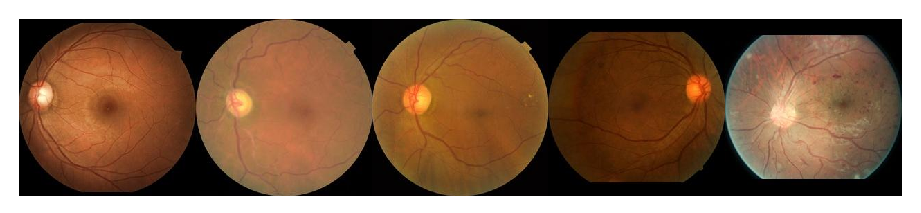
\includegraphics[width=0.55\textwidth]{5classes.eps}
	\caption{0 No Disease, 1 Mild, 2 Moderate, 3 Severe and 4 Proliferative}
\end{figure}

\begin{figure}
	\subfigure{\includegraphics[width=0.3\textwidth]{testing-crop.pdf}}
	\subfigure{\includegraphics[width=0.3\textwidth]{combination-crop.pdf}}
	\caption{Final predictive model}
\end{figure}

\end{frame}

\end{document}
